\documentclass{beamer}

\usepackage{graphicx}
\usepackage{framed}

\begin{document}
	\begin{frame}
\begin{figure}
\centering

\includegraphics[width=0.7\linewidth]{plotlylogo}
\end{figure}
\end{frame}
%============================================%
\begin{frame}
\frametitle{plotly}
\large		
\begin{figure}
\centering
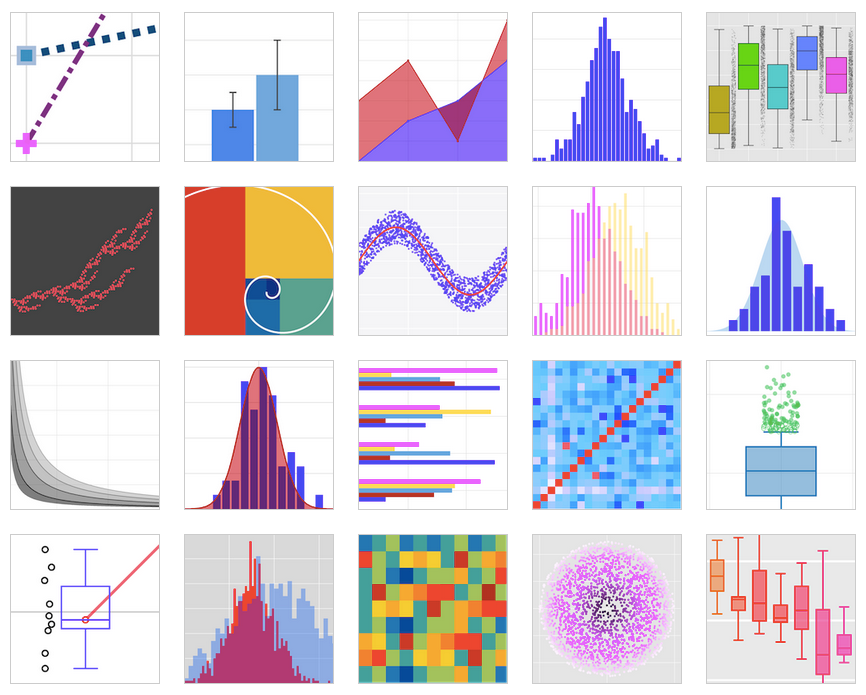
\includegraphics[width=0.7\linewidth]{plotlygallery}
\end{figure}

\end{frame}
%============================================%
\begin{frame}
\frametitle{plotly}
\large	
\begin{itemize}
	\item Plotly is the state of the art in data viz, dashboards, and collaborative analysis, that can be used to make carts and dashboards.
\end{itemize}
\end{frame}

%==================================%
\begin{frame}
\frametitle{plotly}
\large	
\begin{itemize}
	\item Plotly's graphing libraries makes interactive, publication-quality graphs online, with libraries for Python, R, MATLAB, Perl, Julia, Arduino, and REST.
\end{itemize}
\end{frame}
%============================================%

\begin{frame}
Installation
	\begin{figure}
\centering
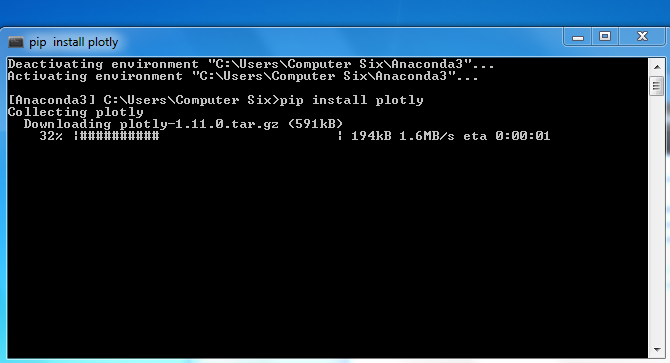
\includegraphics[width=1.1\linewidth]{pipinstallplotly}

\end{figure}

\end{frame}
%=============================================%
\begin{frame}
	\begin{figure}
\centering
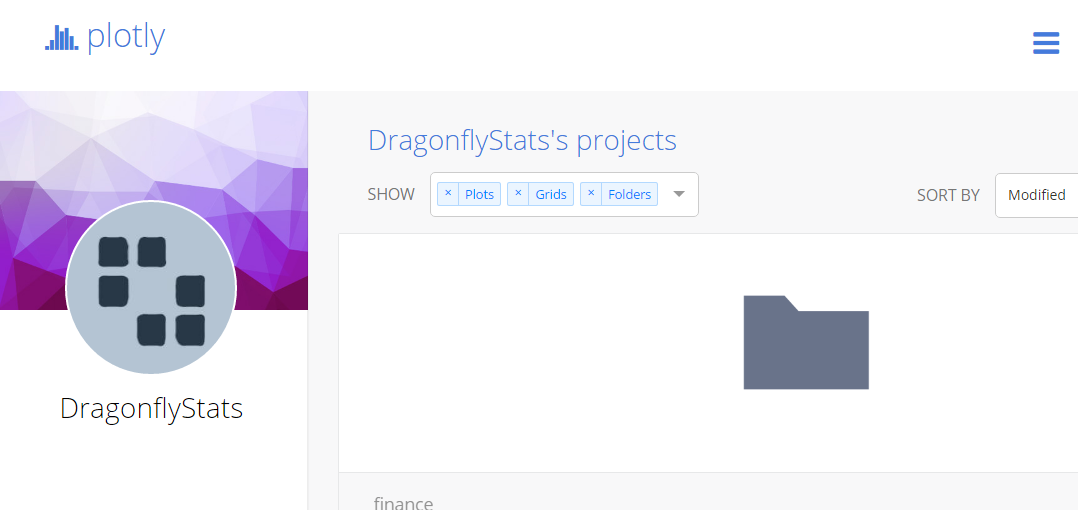
\includegraphics[width=01.1\linewidth]{plotlyprofile}
\end{figure}

\end{frame}
\end{document}
